\section{Adapter Synthesis}
\label{sec:adapter_synthesis}
%
\subsection{Algorithm for Adapter Synthesis}
%
The idea behind CEGIS is to alternate between synthesizing candidate expressions and checking whether those expressions meet a desired specification. 
%
When a candidate expression fails to meet the specification, a counterexample is produced to guide the next synthesis attempt.
%
In our case, the expressions to be synthesized are adapters that map inputs of the target function to inputs of the reference function and outputs of the reference function to outputs of the target function in such a way that the behavior of the two matches. 
%
Our specification for synthesis is provided by the behavior of the target function and we define counterexamples to be inputs on which the behavior of the reference function and target function differ for a given adapter.
%
Our adapter synthesis algorithm is summarized in Figure~\ref{fig:adapter_synthesis}.
%
\begin{figure}[]
\centering
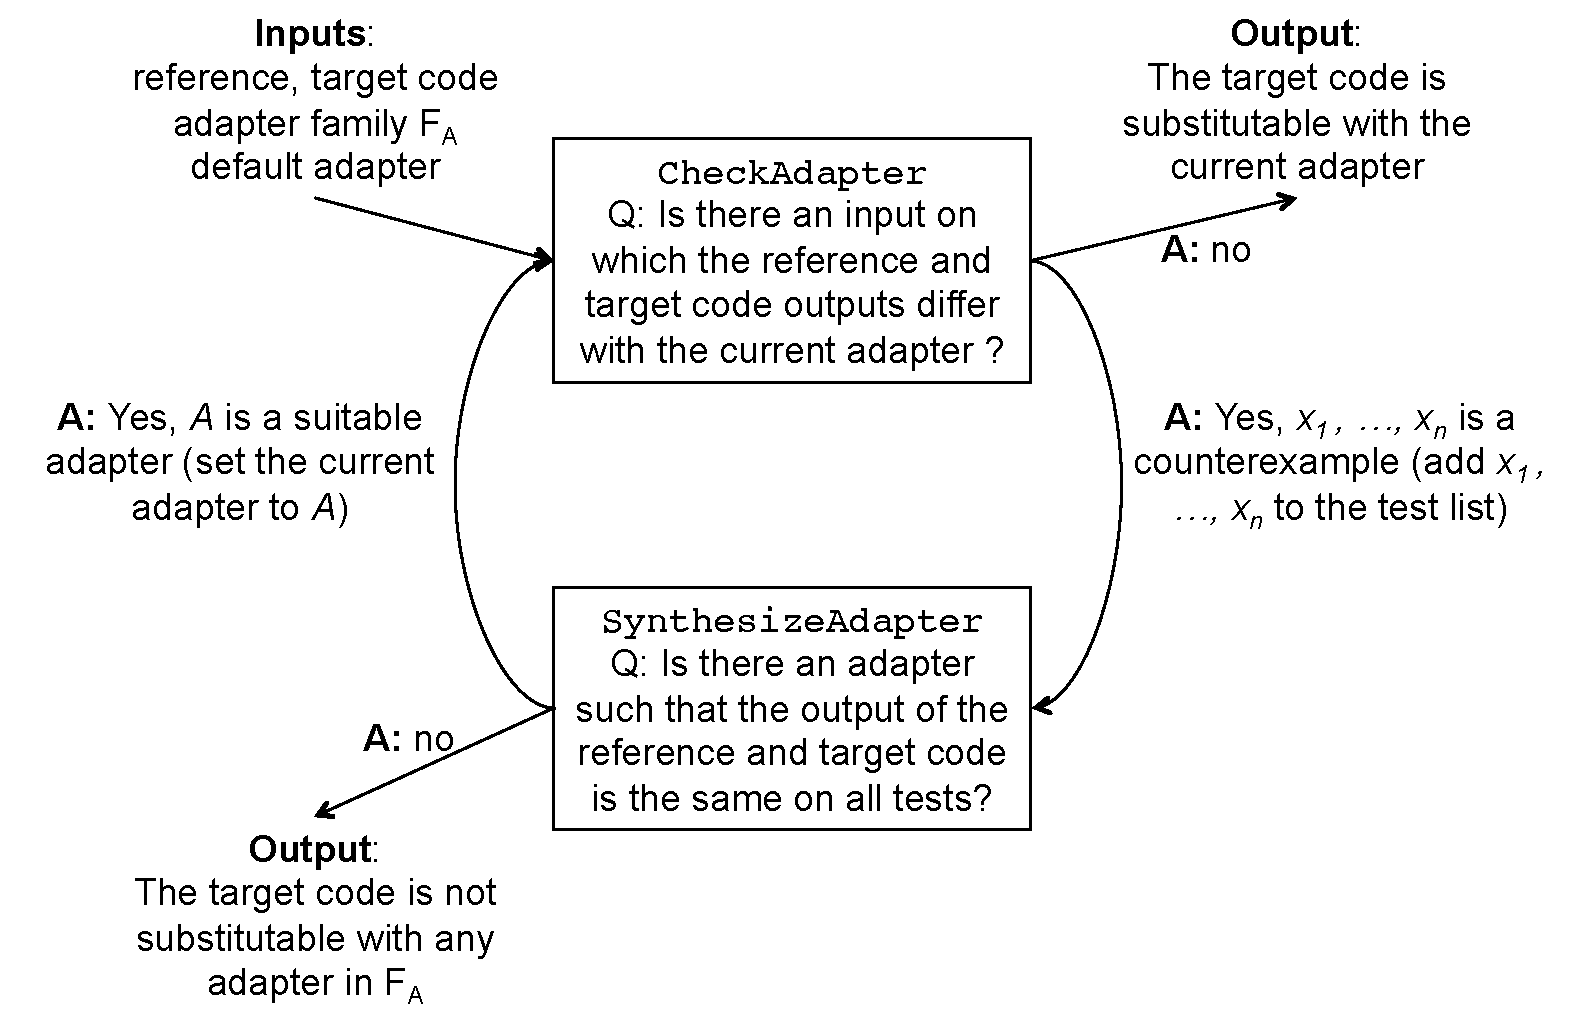
\includegraphics[scale=0.42]{chapters/adapter_synthesis/figures/adapter_synthesis_diagram_v3}
\caption{Counterexample-guided adapter synthesis}
\label{fig:adapter_synthesis}
\end{figure}
%
%More expressive adapters allow for equivalence between more function pairs, but may considerably increase the time required to find a correct adapter.
%
%The adapter grammars we present in the next section represent a trade-off between the desires for generality of adapters and reasonable synthesis performance.
%
As shown in Figure~\ref{fig:adapter_synthesis}, our algorithm takes as input the reference function, the target function, and an adapter family $F_A$. 
%
The algorithm begins with a default adapter and an empty test list.
%
In our implementation, as a default adapter we often use the ``zero adapter,'' which sets every input and output of the reference function to the constant value 0.
%
Until a correct adapter is found or no new adapter can be synthesized, a new counterexample is added to the test list, and any subsequently generated candidate adapters must satisfy all tests in the list.
%
The output of adapter synthesis is either input and output adapters that allow the target function to be substituted by the adapted reference function or an indication that achieving substitutability is not possible using the specified adapter family $F_A$.
%
Our algorithm is guaranteed to terminate if the space of adapters allowed by $F_A$ is finite~\cite{Solar-LezamaTBSS2006}.
%
Although the adapter space and input space may be quite large, in practice we observed that, often, when an adapter was found, the number of steps required to find an adapter was small (see Section~\ref{subsec:eval_general}).

To generate counterexamples and candidate adapters, our adapter synthesis algorithm uses procedures \texttt{CheckAdapter}
and \texttt{SynthesizeAdapter}, which both rely on symbolic execution.
%
\texttt{CheckAdapter} uses symbolic execution to find an input value on which the target function and reference
function outputs disagree with a given adapter and \texttt{SynthesizeAdapter} uses symbolic execution to search for
adapters that cause the target function and reference function to have equivalent output on all inputs in the current test list.
%
Algorithm~\ref{alg:adapter_synthesis} presents the main adapter synthesis loop, Algorithm~\ref{alg:ce_search} presents
the \texttt{CheckAdapter} procedure that generates counterexamples, and Algorithm~\ref{alg:adapter_search} presents
the \texttt{SynthesizeAdapter} procedure that generates candidate adapters.
%
\texttt{CheckAdapter} and \texttt{SynthesizeAdapter} are both implemented as calls to a symbolic executor.
%
%\subsubsection{Algorithms for Adapter Synthesis}
%\label{sec:algorithms}
%Here we present the pseudocode for our adapter synthesis algorithm, which was summarized by Figure~\ref{fig:adapter_synthesis} in Section~\ref{sec:adapter_synthesis}. Algorithm~\ref{alg:adapter_search} presents the main adapter synthesis loop, Algorithm~\ref{alg:check_adapter} presents the \texttt{CheckAdapter} procedure that generates counterexamples, and Algorithm~\ref{alg:synthesize_adapter} presents the the \texttt{SynthesizeAdapter} procedure that generates candidate adapters. \texttt{CheckAdapter} and \texttt{SynthesizeAdapter} are both implemented as calls to a symbolic executor.

\begin{algorithm}[ht]
\LinesNumbered
\small
\SetNlSty{texttt}{[}{]}
\SetKwData{CEList}{test-list}
\SetKwData{CE}{counterexample}
\SetKwFunction{SynthesizeAdapter}{SynthesizeAdapter}
\SetKwFunction{CheckAdapter}{CheckAdapter}
\SetKwInOut{Input}{Input}\SetKwInOut{Output}{Output}
\Input{Target  $T$ as a code fragment or a function, reference function $R$, and adapter family $\mathcal{F}_\mathcal{A}$}
\Output{(input adapter $\mathcal{A}_{in}$, output adapter $\mathcal{A}_{out}$) or \textit{null}}
$\mathcal{A}_{in} \leftarrow$ default-input-adapter\;
$\mathcal{A}_{out} \leftarrow$ default-output-adapter\;
\CEList$\leftarrow$empty-list\;
\While{true}{
%input-args $\leftarrow$ list of symbolic variables;\\
\CE $\leftarrow$ \CheckAdapter($\mathcal{A}_{in}$, $\mathcal{A}_{out}$);\\
\eIf{\CE is null}{
\Return{$(\mathcal{A}_{in}, \mathcal{A}_{out})$\;}
}{
\CEList.append(\CE)\;
}
$(\mathcal{A}_{in}, \mathcal{A}_{out}) \leftarrow$ \SynthesizeAdapter(\CEList)\;
\If{$\mathcal{A}_{in}$ is null}{
\Return{\textit{null}\;}
}
}
\caption{Counterexample-guided adapter synthesis}
\label{alg:adapter_synthesis}
\end{algorithm}

\begin{algorithm}[ht]
\small
\LinesNumbered
\SetNlSty{texttt}{[}{]}
\SetKwInOut{Input}{Input}
\SetKwInOut{Output}{Output}
\Input{Concrete input adapter $\mathcal{A}_{in}$ and output adapter $\mathcal{A}_{out}$}
\Output{Counterexample to the given adapters or \textit{null}}
\SetKwData{args}{args}
\SetKwData{tOut}{target-output}
\SetKwData{rOut}{reference-output}
\args $\leftarrow$ symbolic\;
\While{execution path available} {
%execute a path through the target and inner functions using \args\;
\tOut $\leftarrow$ execute $T$ with input \args\;
\rOut $\leftarrow$ execute $R$ with input \textit{adapt($\mathcal{A}_{in}$, \args)}\;
%solve for concrete \args which create behavioral difference between target and inner function using concrete \fAdapter\;
\If{ ! equivalent(\tOut, adapt($\mathcal{A}_{out}$, \rOut)) }{
\Return{concretize(\args)\;}
}
}
\Return{null\;}
\caption{\texttt{CheckAdapter} procedure used by Algorithm~\ref{alg:adapter_synthesis}. $T$ and $R$ are as defined in Algorithm~\ref{alg:adapter_synthesis}.}
\label{alg:ce_search}
\end{algorithm}

%
\begin{algorithm}[ht]
\LinesNumbered
\small
\SetNlSty{texttt}{[}{]}
\SetKwInOut{Input}{Input}
\SetKwInOut{Output}{Output}
\SetKwData{CEList}{test-list}
\SetKwData{CE}{test}
\SetKwData{tOut}{target-output}
\SetKwData{rOut}{reference-output}
\SetKwData{eqCounter}{eq-counter}
\Input{List of previously generated counterexamples \CEList}
\Output{(input adapter $\mathcal{A}_{in}$, output adapters $\mathcal{A}_{out}$) or \textit{null}}
$\mathcal{A}_{in} \leftarrow$ symbolic input adapter\;
$\mathcal{A}_{out} \leftarrow$ symbolic output adapter\;
\While{execution path available} {
\eqCounter $\leftarrow$ 0\;
\While{\eqCounter $<$ length(\CEList)} {
%execute a path through the target and inner functions using \CE\;
\tOut $\leftarrow$ execute $T$ with input \CE\;
\rOut $\leftarrow$ execute $R$ with input adapt($\mathcal{A}_{in}$, \CE))\;
%solve for concrete \adapter which gives behavioral equivalence between target and inner function\;
\eIf{ equivalent(\tOut, adapt($\mathcal{A}_{out}$, \rOut))}{
\eqCounter $\leftarrow$ \eqCounter + 1\;
} {break\;}
}
\If{ \eqCounter == length(\CEList) }{
\Return{(concretize($\mathcal{A}_{in}$), concretize($\mathcal{A}_{out}$))\;}
}
}
\Return{null\;}
\caption{\texttt{SynthesizeAdapter} procedure used by Algorithm~\ref{alg:adapter_synthesis}. $T$ and $R$ are as defined in Algorithm~\ref{alg:adapter_synthesis}. The form of the resulting adapters ($\mathcal{A}_{in}$, $\mathcal{A}_{out}$) is dictated by $\mathcal{F}_\mathcal{A}.$}
\label{alg:adapter_search}
\end{algorithm}
%

Adapter synthesis terminates when either \texttt{CheckAdapter} or \texttt{SynthesizeAdapter} have explored every available execution path without finding a counterexample or new candidate adapter.
%
If \texttt{CheckAdapter}  fails to find a counterexample, we conclude that the current adapter allows the target function to be substituted by the reference function.
%
If \texttt{SynthesizeAdapter}  fails to generate an adapter, we conclude that the target function is not substitutable by the reference function with any adapter in $F_A$.
%
%The ability of the symbolic executor to get full path coverage depends both on the program being executed and the size of $\mathcal{F}_\mathcal{A}$.
%
If either \texttt{CheckAdapter} or \texttt{SynthesizeAdapter} fail due to a timeout, we make no claims about the substitutability of the target function by the adapted reference function.
However, our observation from our evaluation is that the majority of adapter synthesis tasks that timed out would eventually lead to the conclusion of no possible adapter.
%
We explore timeouts in more detail in Section~\ref{subsec:eval_general}.
%
\subsection{Adapter Families}
The \texttt{SynthesizeAdapter} step synthesizes an adapter from a finite family of adapters. 
%
We currently support the following families of adapters, of which the arithmetic and memory substitution adapter families are newly introduced in this work.
%
\subsubsection{Argument Substitution}
This family of adapters allows replacement of any reference function argument by one of the target function arguments or a constant.
% Listing \ref{lst:simple_adapter} presents an adapter that can be synthesized using simple argument substitution.
% While this pair of function is not derived from real-world software, this is an interesting example because the functions \textit{$f_1$} and \textit{$f_2$} have a non-intuitive relationship, and it is not immediately obvious that they are equivalent.
This family is useful, for instance, when synthesizing adapters between the cluster of functions in the C library that wrap around the \textit{wait} system call as shown in Section \ref{subsec:c-library-evaluation}.
% 
%\lstinputlisting[caption={Simple argument substitution adapter example}, label={lst:simple_adapter}, style=nonumbers]{code_samples/simple.c}
%
% \textbf{Argument Substitution with String Length:} 
% This family extends the argument substitution adapter family by adding the ability to replace an inner function argument by the length (as computed by \textit{strlen}) of a target function argument. 
% %
% For instance, the C library function \textit{fwrite} can be adapted to \textit{fputs} by setting its second argument to the constant 1 and its third argument to the length of its first argument.\\
% %
\subsubsection{Argument Substitution with Type Conversion}
This family extends the argument substitution adapter family by allowing
reference function arguments to be the result of a type conversion applied to a target function argument. 
%
Since type information is not available at the binary level, this adapter tries all possible combinations of type conversion on function arguments.
%
Applying a type conversion at the 64-bit binary level means that each
target function argument itself may have been a \textit{char},
\textit{short} or a \textit{int}, thereby using only the low 8, 16, or
32 bits respectively of the argument register.
%
The correct corresponding reference function argument could be produced by either a sign extension or zero extension on the low 8, 16, or 32 bits of the argument register. 
%
%Listing \ref{lst:typeconv} presents an additional adapter that can be synthesized for the target and inner functions in Listing \ref{lst:simple_adapter} when type conversions on target function arguments are allowed during adapter search. 
%The $y \& 1$ expression represents a 1-bit zero-extension operation.
This adapter family also allows for converting target function arguments to boolean values by comparing those arguments to zero. 
\subsubsection{Arithmetic adapter}
%
This family allows reference function arguments to be arithmetic combinations of target function arguments.
%
This adapter family has been implemented by Hietala~\cite{kesha-thesis}.
%
%\lstinputlisting[caption={Type conversion adapter for the function pair shown in Listing \ref{lst:simple_adapter}}, label={lst:typeconv}, style=nonumbers]{code_samples/typeconv.c}
\subsubsection{Memory Substitution}
This family of adapters allows a field of a reference function structure argument to be adapted to a field of a target function structure argument.
%
Each field is treated as an array with \textit{n} entries (where $n \geq
1$), with each entry of size 1, 2, 4, or 8 bytes.
%
Corresponding array entries used by the target and reference functions need not be at the same address and may also have different sizes, in which case both sign-extension and zero-extension are valid options to explore for synthesizing the correct adapter as shown in Figure~\ref{fig:memsub}.
%
This makes our adapter synthesis more powerful because it can be used in
combination with other adapter families that allow argument substitution. 
%
This adapter family synthesizes correct adapters between RC4 implementations in the mbedTLS and OpenSSL libraries in Section~\ref{subsec:rc4-experiment}.
%
\begin{figure}[h]
\caption{Memory substitution adapter to make \textit{struct r} adaptably equivalent to \textit{struct t}}
\label{fig:memsub}
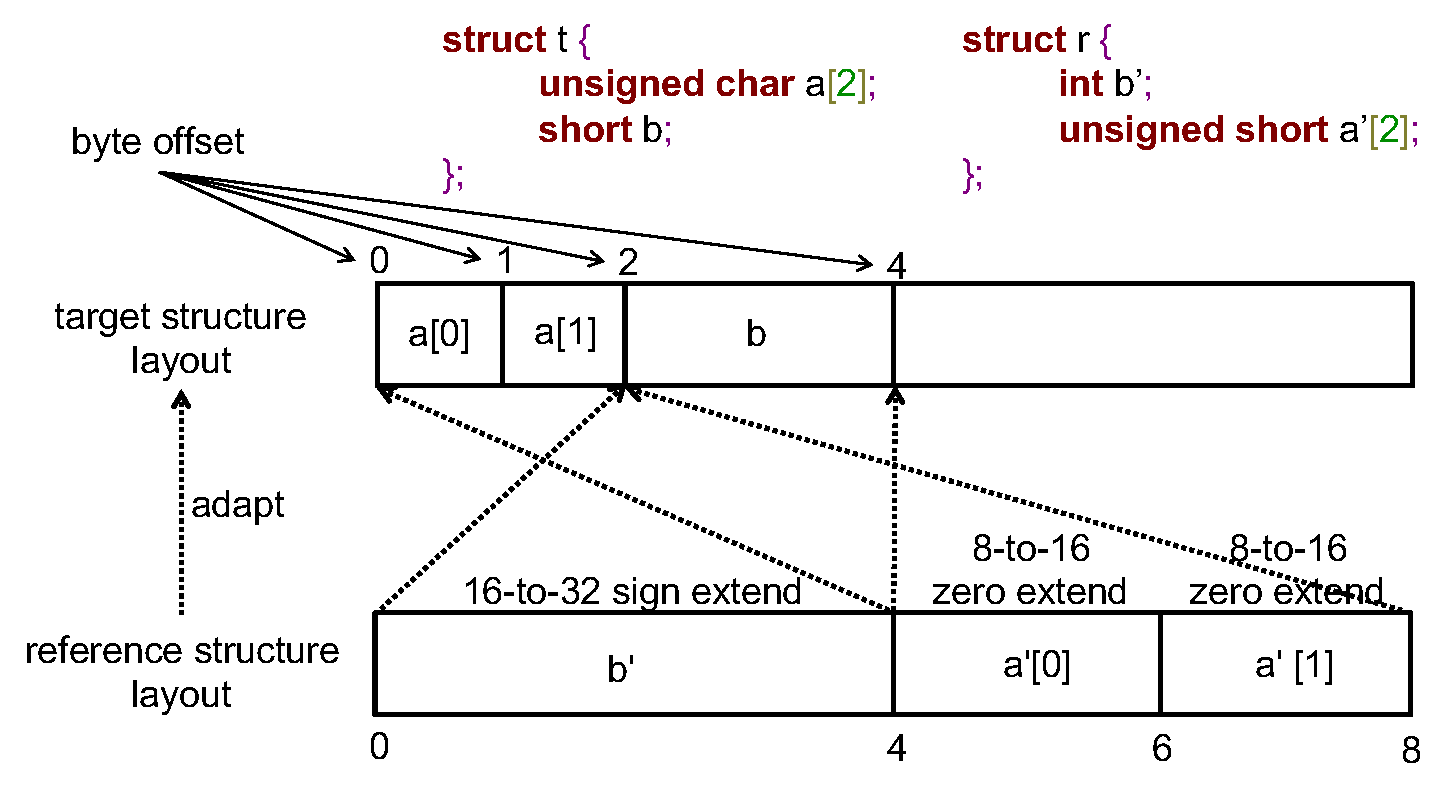
\includegraphics[width=\widthfactor\columnwidth]{chapters/adapter_synthesis/figures/memsub_pdf6}
\end{figure}  
\subsubsection{Return Value Substitution}
The argument substitution families described above can also be applied on return values.
%
An example of different return values having the same semantic meaning is the return value of the C library function \textit{isalpha} as shown in Listing \ref{lst:isalpha}.
%
The wrapper function \textit{adapted\_isalpha} in Listing~\ref{lst:isalpha} performs
return value substitution.
%
%As per the C library specification, the functions \textit{isalpha}, \textit{isalnum} must return a non-zero value if their argument is a digit, a alphabet, or a alphanumeric character respectively, and return zero otherwise.
%
%While any non-zero return value for these two functions has the same semantic meaning, when these predicates are satisfied, the eglibc library implementation~(the system C library commonly available on Ubuntu 14.04) of these two functions returns non-zero values from these two functions that are different from those returned by the musl, a newer implementation of the C library specification.
%
%This example provides motivation for this family of adapters because changing a nonzero return value of such predicate functions to 1 harmonizes the difference between return values of the same isalpha predicate. \\ %can create functional equivalence as shown in Listing \ref{lst:return_adapter}. 
%
%\lstinputlisting[caption={Return value substitution adapter example}, label={lst:return_adapter}, style=nonumbers]{code_samples/return-adapter.c}
%
%This is shown in Listing \ref{lst:arithmetic_bit_synthesis}. 
%\lstinputlisting[caption={Arithmetic adapter example}, label={lst:arithmetic_bit_synthesis}, style=nonumbers]{code_samples/arithmetic-bit-synthesis.c}
%    \textbf{Character Set Translation adapter:}
%    %\subsubsection{Character Set Translation adapter}
%    The \textit{chartrans} rule in Grammar \ref{grammars} translates each character according to some fixed mapping.
%    The \textit{tr} function provides character set translations similar to the \texttt{tr} Unix utility (without squeezing or deleting characters) in string arguments.
%    The \textit{LIST1} and \textit{LIST2} terminals in the \textit{chartrans} rule specify the source-to-destination mapping.
%    e.g. the first character in \textit{LIST1} is translated to the first character in \textit{LIST2}.
%    \todo{example ?}
%Listing \ref{lst:chartrans_adapter} shows an example application of this adapter grammar. 
%While both \textit{$f_1$} and \textit{$f_2$} check whether a the input string is a palindrome, \textit{$f_1$} expects the string to be newline-terminated and \textit{$f_2$} expects the string string to be null-terminated. 
%The adapter between \textit{$f_1$} and \textit{$f_2$} translates every instance of the newline character to the null character.

% \lstinputlisting[caption={Character set translation adapter example}, label={lst:chartrans_adapter}, style=nonumbers]{code_samples/chartrans-adapter.c}

\subsection{Example}
%
\begin{figure}
\lstinputlisting[caption={Two implementations of similar adaptable functionality}, label={lst:example}, style=nonumbers]{chapters/adapter_synthesis/code_samples/example.c}
\end{figure}
%
To illustrate our approach, we walk through a representative run of our adapter synthesis algorithm using a pair of target and reference functions that implement similar functionality.
%
Both the target and reference functions are shown in Listing~\ref{lst:example}. 
%
Here we will focus only on synthesis of the input adapter, although the general algorithm also produces an adapter that adapts the output of the reference function. 
%
A correct input adapter should set the first argument of \texttt{reference} to the integer argument $y$ of \texttt{target} and set the second argument to the constant 1 to adaptably substitute the \texttt{y \% 2} operation in \texttt{target}.
%
It should also set both the third and fourth arguments of \texttt{reference} to the first argument of \texttt{target} to adaptably substitute the \texttt{x << 1} operation in \texttt{target}. 
%
We write this adapter as $\mathcal{A}(x,y) = (y, 1, x, x)$.

\textbf{Step 0:} 
Adapter synthesis begins with an empty counterexample list and a default adapter that maps every argument to the constant 0 (i.e. $\mathcal{A}(x,y) = (0,0,0,0)$). During counterexample generation (\texttt{CheckAdapter} in Figure~\ref{fig:adapter_synthesis}), we use symbolic execution to search for an inputs $x,y$ such that the output of \texttt{target(x,y)} is not equivalent to the output of \texttt{reference(}$\mathcal{A}(x,y)$\texttt{)} = \texttt{reference(0,0,0,0)}. From \texttt{CheckAdapter}, we learn that $x = 1, y = 0$ is one such counterexample.
 
\textbf{Step 1:} Next, during adapter search (\texttt{SynthesizeAdapter} in Figure~\ref{fig:adapter_synthesis}), we use symbolic execution to search for a new adapter $\mathcal{A}$ that will make \texttt{target(x)} equivalent to \texttt{reference(}$\mathcal{A}(x,y)$\texttt{)} for all inputs $x,y$ in the list [(1,0)]. From \texttt{SynthesizeAdapter}, we learn that $\mathcal{A}(x,y) = (y,y,x,x)$ is a suitable adapter, and this becomes our new current adapter.

\textbf{Step 2:} We use \texttt{CheckAdapter} to search for a counterexample to the current adapter, $\mathcal{A}(x,y) = (y,y,x,x)$. We find that $x = 0, y = 3$ is a counterexample. 

\textbf{Step 3:} Next, we use \texttt{SynthesizeAdapter} to search for
an adapter $\mathcal{A}$ for which the output of \texttt{target(x)} will
be equivalent to the output of
\texttt{reference(}$\mathcal{A}(x,y)$\texttt{)} for both pairs of
inputs, $x = 1, y = 0$ and $x = 0, y = 3$. \texttt{SynthesizeAdapter} identifies $\mathcal{A}(x) = (y,1,x,x)$ as a suitable adapter.

\textbf{Step 4:}
At the beginning of this step, the current adapter is $\mathcal{A}(x,y) = (y,1,x,x)$. As before, we use \texttt{CheckAdapter} to search for a counterexample to the current adapter. We find that \texttt{CheckAdapter} fails to find a counterexample for the current adapter, indicating that the current adapter is correct for all explored paths. Therefore, adapter synthesis terminates with the final adapter $\mathcal{A}(x) = (y, 1, x, x)$.
%Alternatively, adapter synthesis could have terminated with the decision that the target function is not substitutable by the reference function with any allowed adapter.
%In our evaluations, adapter synthesis may also terminate with a timeout, indicating the total runtime has exceeded a predefined threshold.

\subsection{Extensibility}

The adapter synthesis algorithm presented in this section is not tied to a source programming language or adapter family.
In our implementation (Section~\ref{sec:implementation}) we target
binary x86 and ARM code, and we use adapters that allow for common
argument structure changes found in binaries compiled from C and C++ code.
Because we work at the binary level, we are also not restricted to working at the level of target functions as described so far.
In Section~\ref{subsec:eval_general}, instead of target functions, we consider target ``code fragments.''
We define a code fragment to be a sequence of instructions consisting of at least one instruction. 
Inputs to code fragments are the general-purpose registers available on the architecture of the code fragment and outputs are registers written to within the code fragment.
%
We could similarly allow reference functions to be more general code regions.

